% Draft vCage paper.
% Format based on official ACM template.

% Use ACM official template.  Either OK for submission, but
% sig-alternate produces tighter, better-looking output.
\documentclass{sig-alternate}
% \documentclass{acm_proc_article-sp}
\usepackage{graphicx}
\graphicspath{ {./figures/} }


% Some useful macros.

% time macros
\newcount\hour
\newcount\minute
\hour=\time
\divide \hour by 60
\minute=\time
\loop \ifnum \minute > 59 \advance \minute by -60 \repeat
\def\now{%
\ifnum \hour<13
\ifnum \hour<1 12:\else\number\hour:\fi
\ifnum \minute<10 0\fi
\number\minute%
\ifnum \hour<12 \ am \else \ pm \fi
\else \advance \hour by -12 \number\hour:%
\ifnum \minute<10 0\fi
\number\minute%
\ pm \fi%
}

% project name (use macro to facilitate renaming)
\newcommand{\vcage}{vCage}


\begin{document}

% Tentative title.
\title{A Software Cryptoprocessor for Commodity Servers}

%
% You need the command \numberofauthors to handle the 'placement
% and alignment' of the authors beneath the title.
%
% For aesthetic reasons, we recommend 'three authors at a time'
% i.e. three 'name/affiliation blocks' be placed beneath the title.
%
% NOTE: You are NOT restricted in how many 'rows' of
% "name/affiliations" may appear. We just ask that you restrict
% the number of 'columns' to three.
%
% Because of the available 'opening page real-estate'
% we ask you to refrain from putting more than six authors
% (two rows with three columns) beneath the article title.
% More than six makes the first-page appear very cluttered indeed.
%
% Use the \alignauthor commands to handle the names
% and affiliations for an 'aesthetic maximum' of six authors.
% Add names, affiliations, addresses for
% the seventh etc. author(s) as the argument for the
% \additionalauthors command.
% These 'additional authors' will be output/set for you
% without further effort on your part as the last section in
% the body of your article BEFORE References or any Appendices.

%% \numberofauthors{8} %  in this sample file, there are a *total*
%% % of EIGHT authors. SIX appear on the 'first-page' (for formatting
%% % reasons) and the remaining two appear in the \additionalauthors section.
%% %
%%
%% \author{
%% % You can go ahead and credit any number of authors here,
%% % e.g. one 'row of three' or two rows (consisting of one row of three
%% % and a second row of one, two or three).
%% %
%% % The command \alignauthor (no curly braces needed) should
%% % precede each author name, affiliation/snail-mail address and
%% % e-mail address. Additionally, tag each line of
%% % affiliation/address with \affaddr, and tag the
%% % e-mail address with \email.
%% %
%% % 1st. author
%% \alignauthor
%% Ben Trovato\titlenote{Dr.~Trovato insisted his name be first.}\\
%%        \affaddr{Institute for Clarity in Documentation}\\
%%        \affaddr{1932 Wallamaloo Lane}\\
%%        \affaddr{Wallamaloo, New Zealand}\\
%%        \email{trovato@corporation.com}
%% % 2nd. author
%% \alignauthor
%% G.K.M. Tobin\titlenote{The secretary disavows
%% any knowledge of this author's actions.}\\
%%        \affaddr{Institute for Clarity in Documentation}\\
%%        \affaddr{P.O. Box 1212}\\
%%        \affaddr{Dublin, Ohio 43017-6221}\\
%%        \email{webmaster@marysville-ohio.com}
%% % 3rd. author
%% \alignauthor Lars Th{\o}rv{\"a}ld\titlenote{This author is the
%% one who did all the really hard work.}\\
%%        \affaddr{The Th{\o}rv{\"a}ld Group}\\
%%        \affaddr{1 Th{\o}rv{\"a}ld Circle}\\
%%        \affaddr{Hekla, Iceland}\\
%%        \email{larst@affiliation.org}
%% \and  % use '\and' if you need 'another row' of author names
%% % 4th. author
%% \alignauthor Lawrence P. Leipuner\\
%%        \affaddr{Brookhaven Laboratories}\\
%%        \affaddr{Brookhaven National Lab}\\
%%        \affaddr{P.O. Box 5000}\\
%%        \email{lleipuner@researchlabs.org}
%% % 5th. author
%% \alignauthor Sean Fogarty\\
%%        \affaddr{NASA Ames Research Center}\\
%%        \affaddr{Moffett Field}\\
%%        \affaddr{California 94035}\\
%%        \email{fogartys@amesres.org}
%% % 6th. author
%% \alignauthor Charles Palmer\\
%%        \affaddr{Palmer Research Laboratories}\\
%%        \affaddr{8600 Datapoint Drive}\\
%%        \affaddr{San Antonio, Texas 78229}\\
%%        \email{cpalmer@prl.com}
%% }
%% % There's nothing stopping you putting the seventh, eighth, etc.
%% % author on the opening page (as the 'third row') but we ask,
%% % for aesthetic reasons that you place these 'additional authors'
%% % in the \additional authors block, viz.
%% \additionalauthors{Additional authors: John Smith (The Th{\o}rv{\"a}ld Group,
%% email: {\texttt{jsmith@affiliation.org}}) and Julius P.~Kumquat
%% (The Kumquat Consortium, email: {\texttt{jpkumquat@consortium.net}}).}
%% \date{30 July 1999}
%% % Just remember to make sure that the TOTAL number of authors
%% % is the number that will appear on the first page PLUS the
%% % number that will appear in the \additionalauthors section.

% Anonymous submission.
\numberofauthors{1}
\author{Authors omitted for blind review}
\toappear{Draft in preparation for submission to ACM CCS '14.\\
Generated \today\ at \now\\
Confidential --- Do Not Distribute}

\maketitle

% Abstract
\begin{abstract}
\label{sec:abstract}

Defending computers from unauthorized physical access and malicious
hardware devices has proved extremely challenging.  The problem is
exacerbated in cloud-computing environments, where users lack physical
control over the server hardware that executes their workloads.
Moreover, cloud service providers can be compelled by government
agencies to provide physical access to servers.

We introduce {\em \vcage}, a software-based cryptoprocessor system
that employs cryptographic techniques to provide confidentiality for
unmodified workloads. Code and data are stored as cleartext only
within the processor cache, but remain encrypted in main memory.  We
implemented \vcage\ in a commercial product for commodity server
platforms based on Intel x86 processors and industry-standard TPMs.

We present the design and implementation of \vcage\ in Linux, and show
how it virtualizes physical security by protecting data-in-use
transparently for KVM virtual machines.  Quantitative experiments
demonstrate that \vcage\ effectively safeguards privacy, while
achieving acceptable performance for a wide range of workloads.


\end{abstract}

% Tentative categories (required).
\category{D.2.6}{Operating Systems}{Security and Protection}
\terms{Security}
\keywords{Memory Protection, Processor Cache, Operating Systems,
Hypervisors, Virtual Machines}

% Use separate file for each section to facilitate concurrent editing.
\section{Introduction}
\label{sec:intro}

Introduction goes here...

\section{Physical Attacks}
\label{sec:physical}

It is generally understood that physical access to an x86 platform can
completely compromise software security. Historically, physical
security controls, such as cages, cameras, and locks, have been employed to
prevent or detect physical access. Yet with adoption of
outsourced infrastructure and cloud computing, x86 platforms are
increasingly run outside the physical control of the software owner.

This section briefly summarizes several well-known physical attack vectors
against x86 platforms, including DMA, physical memory extraction, and
platform malware.

\subsection{Direct Memory Access}

By design, x86 architectures provide direct memory access (DMA) from
hardware subsystems to access main memory independently of the
CPU. DMA access is generally used for performance, for example
allowing disk, network, and graphics devices to read and write
data directly to memory without incurring CPU cycles.

Yet, without proper controls, devices with DMA access can read
arbitrary regions of memory and compromise system security by exposing
secrets or allowing an attacker to modify running software in
place. Secrets from captured memory can be extracted easily with
forensics tools like Volatility \cite{Volatility:2014}.

Tribble \cite{Carrier:2004hardware, Grand:2007patent} is an
early example of a device desiged for exfiltrating data via DMA
access, based on an off-the-shelf Intel development kit. Copilot
\cite{Petroni:2004copilot} also used DMA with a PCI device for the
purpose of monitoring kernel integrity. The Maux attack
\cite{Triulzi:2008vd} exploited remote vulnerabilities in a standard
network interface device and accessed memory via DMA. Off-the-shelf
intelligent network adapters, such as those made by Cavium, are able
to exfiltrate DMA-accessed memory over a network connection
\cite{Horovitz:2013physical}.

The IEEE 1394 Firewire interface also provides DMA by design. This led
to several demonstrations of memory extraction to steal data or for
forensics \cite{Dornseif:20040wned, Boileau:2006we,
  Witherden:2010forensics, Dornseif:2005firewire}. The Thunderbolt
interface also offers DMA access and can be exploited in a similar
manner \cite{Maartmann:2011inception}.

\subsection{Physical Memory Extraction}

While DMA may be mitigated by software-based countermeasures,
leveraging a hardware IOMMU such as
Intel VT-d \cite{Intel-IOMMU:2013}, other attacks involve the physical
extraction or modification of system memory. For example, memory bus
analyzer devices are available and can interdict memory
traffic. However, bus analyzers must be installed ahead of time, tend
to be relatively expensive, and physically large.

A ``cold boot'' is a low-cost memory extraction attack that can be
conducted for little cost on a running system
\cite{Halderman:2008tp}. Cold booting involves literally freezing
system memory modules with an aerosol freeze spray. The memory
contents are preserved long enough to boot to a ``scraper'' image such
as {\em bios-memimage} or {\em msramdump} which can preserve the
memory contents to persistent storage.

Cold booting disrupts a running system and data must be recovered
immediately, before the memory module thaws. Furthermore, it does not
reliably capture all memory contents, as there is some degradation
over time. Conducting the attack may be further complicated by
error-correcting memory which is cleared on a reset or by data
scrambling for power supply noise suppression \cite{Mozak:2011lfsr}.

Non-volatile memory (NV-RAM), designed to persist data after a power
loss, is now available in DDR3/DDR4 form-factors used by standard x86
servers. An attacker can install NV-RAM modules in a server and remove
them at any moment, recovering the data at a later time. If a memory
mirroring mode is configured, an attacker could remove a NV-RAM module
from a running system and replace it without disrupting service.


\subsection{Bootkits and Platform Malware}

\begin{itemize}
  \item APT
\end{itemize}

\subsection{Practical Attack Vectors}

{\em SW: This might be unnecessary. Do we really need to explain how people get
physical access? }

{\em CW: Suggest writing a few sentences, and moving to intro for this
section.  The NSA attacks seem particularly interesting to at least mention.}

\begin{itemize}
  \item Supply chain
  \item Datacenter insiders
  \item Previous bare-metal host tenants: Can we pwn our SoftLayer BIOS?
  \item Stoned bootkit in the wild
  \item NSA ANT
\end{itemize}

\section{Cache Management}

Compared to a conventional system, \vcage\ treats the processor cache
like main memory, and main memory like an encrypted backing store.
All cleartext data must remain resident in the processor cache for
correctness; evictions could leak sensitive data to untrusted main
memory.  Since cache space is smaller than traditional main memory
sizes by orders of magnitude, it must be managed efficiently.

Fortunately, cache sizes are growing rapidly along with advances in
process technology.  Modern multi-core processors integrate a large,
physically-indexed last-level cache (LLC) shared among multiple cores.
Currently, the Intel Ivy Bridge EX x86 processor is available with a
37.5MB on-die LLC.  Unfortunately, x86 processors lack hardware
support for explicit software control over cache allocation and
eviction policies.  Moreover, recent x86 hardware introduced complex
cache indexing, which makes software cache management even more
difficult.

After reviewing processor caching behavior, including memory types and
cache indexing, we explain how \vcage\ manages cache contents despite
numerous challenges.

\subsection{Memory Types}

Processors commonly provide some method for specifying how regions of
physical memory should be cached.  The x86 architecture
\cite{Intel-SDM} supports a small set of memory type range registers
(MTRRs), each of which can be programmed to control the caching method
used for a contiguous region of memory, subject to various size and
alignment constraints.  A similar capability is provided for
specifying caching attributes of individal pages via page tables
entries and the x86 page attribute table (PAT).

\vcage\ uses MTRRs to prevent nearly all of untrusted main memory from
being cached, setting the memory type to {\em write-combining (WC)},
instead of {\em uncacheable (UC)}. Neither memory type is cached, but
WC offers significantly higher performance than UC, due to load and
store buffering.  However, write combining uses a weak memory ordering
model which is not appropriate for general-purpose data; in most
systems, it is used only for video frame buffers.  \vcage\ accesses WC
memory in a controlled manner for encrypted paging.  Data is copied
between the cache and memory using non-temporal move instructions
that utilize write-combining store buffers and streaming load buffers
efficiently \cite{Intel-SDM}.

\subsection{Traditional Cache Indexing}

Memory is cached in units of {\em lines}; on modern x86 hardware, the
cache line granularity is 64 bytes, with 64-byte alignment.  The
processor maps each line of memory to a single $n$-way associative
{\em cache set} based on its physical address.  For example, on the
Intel Sandy Bridge x86 processor, a single last-level cache set
consists of 20 lines; {\em i.e.}, the cache is 20-way set associative.

Main memory is normally several orders of magnitude larger than the
cache, so many more than $n$ lines of physical memory map to the
same cache set.  When a new line of memory needs to be cached in a set
that is already full, these {\em conflicting} lines contend for the
same scarce cache space.  The processor implements a cache replacement
policy that chooses some existing line to replace, typically evicting
one of the least recently used (LRU) lines from the set to optimize
for temporal locality.

Traditionally, processors have employed a simple mapping of physical
addresses to cache sets, based on lower-order bits of the physical
address.  For example, consider an Intel Nehalem x86 processor with an
8MB 16-way set-associative cache.  Each cache set contains 16 lines
$\times$ 64B = 1KB of cached data; the entire cache contains 8K sets,
requiring a 13-bit index.  A physical address is mapped to a cache set
using bits 6..18 as the cache set index, with bits 0..5 specifying the
intra-line byte offset.

\subsection{Page Coloring}

When paging is used for address translation, the low-order bits of the
physical page number are the high-order bits of the cache set index.
This straightforward hardware mapping of physical addresses to cache
sets has been leveraged for many years by operating systems and
hypervisors, using a technique known as {\em page coloring}.  By
controlling the virtual-to-physical page mapping, system software can
partition pages into disjoint sets, or {\em colors}, such that pages
with different colors do not conflict in the cache.

In the Nehalem example above, there are 128 page colors when using
conventional 4KB x86 ``small'' pages. Bits 0..6 of the physical page
number, corresponding to physical address bits 12..18, specify the
page color -- a contiguous range of sets used to cache the page
contents.

Page coloring has been used in many systems to improve performance by
reducing cache conflict misses \cite{Bugnion-PageColoring}, and to
control the isolation or sharing of cache memory between software
contexts \cite{Zhang-PageColoring}.  Commercial hypervisors have
preserved the relative page coloring used by the guest OS within a
virtual machine \cite{Waldspurger-ESX}.  We had originally intended to
leverage page coloring to enable \vcage\ to manage the processor
cache.  However, as detailed below, recent changes in processor cache
indexing have complicated this approach.

\subsection{Complex Cache Indexing}

Recent Intel x86 processors, starting with the Sandy Bridge
micro-architecture, use a ring-based interconnect between cores and a
multi-banked last level cache (LLC), which is organized into multiple
cache {\em slices}.  Physical addresses are mapped to LLC cache sets
within slices using ``complex cache indexing''
\cite{Intel-Uncore-E5-2600,Intel-SDM}.  The hardware that realizes
this mapping implements an undocumented, proprietary hash function,
and may potentially use any physical address bits as inputs.  The hash
function may also vary across different processor implementations and
configurations.

As a result, traditional page-coloring techniques may no longer work.
A small contiguous memory region can be scattered across many
discontiguous sets throughout the cache.  Since \vcage\ requires
strict control over the cache, we developed a reliable approach for
generating fine-grained address-to-cache-set mappings on modern
Intel processors.

\subsection{Discovering Set Mappings}

We present a programmatic method for computing complete information
about processor-specific mappings from physical addresses to cache
sets. Although we use Intel x86 processors, the same general technique
should work on any architecture with deterministic cache indexing
and accurate cache performance counters.

As input, the method takes a collection of physical addresses at
cache-line granularity, typically a single contiguous address range.
As output, these addresses are partitioned into cache
{\em conflict sets}, such that addresses within a partition conflict
in the cache, and addresses in different partitions do not conflict.
The basic idea is to exceed the limited associativity of a
single $n$-way associative cache set to force observable cache
evictions and discover conflicts.

An empty conflict set $S$ is allocated, and used to maintain an array
of addresses observed to conflict in the LLC.
The entire cache is flushed using the the x86 {\tt WBINVD} instruction
to start from a known empty state.

Loads are issued to each input memory address, one-by-one, until a
hardware performance counter, programmed to monitor LLC evictions, and
checked after each load, detects that a first eviction has occurred.
On the Intel Sandy Bridge and Ivy Bridge processors, the uncore
caching-agent (CBo) performance counters were programmed to monitor
the {\tt LLC\_VICTIMS} event, filtered by the MES cache states
\cite{Intel-Uncore-E5-2600}.  Since lines in different slices cannot
conflict, and the hardware provides per-slice counters, this procedure
is run for each slice independently.  Conveniently, this also
eliminates any potential interference from concurrent cache activity
in other slices.

The address which caused the eviction is added to $S$.  The cache is
again flushed, and loads are performed to all addresses in $S$,
to ensure that they are resident in the cache.  As a result, a
different conflicting input address associated with the same set will
cause the next eviction -- essentially rotating through a ring of
conflicting lines that exceed the hardware cache associativity.  Loads
are issued again to the remaining set of potentially-conflicting input
addresses, one-by-one, in the same order, and the address causing the
next eviction is added to $S$.

This process is repeated until $|S| > n$, or several repetitions yield
addresses already in $S$.  Each generated partition will contain $n+1$
physical lines for an $n$-way set-associative cache.  To support
larger input regions, once a conflict set $S$ contains $n+1$
addresses, one is selected, moved to an ``overflow'' list associated
with $S$, and removed as an active input address.  This process can be
repeated until all input memory addresses have been partitioned into
conflict sets.

After each conflict set is identified, each of its its constituent
addresses is marked as already ``used'' by some set.  When input
addresses are read one-by-one in the method outlined above, any which
have already been marked as used are instead flushed from the cache
using the x86 {\tt CLFLUSH} instruction.  This prevents noise due to
prefetching or eviction events from other sets.

Additional steps can further improve the robustness and accuracy of
this approach, including mapping the primary data structures as
uncached, disabling interrupts during the computation of each
conflict set, disabling prefetching, and booting in uniprocessor mode
to prevent memory accesses from other cores sharing the LLC.  More
generally, multiple runs can be performed to resolve any discrepancies
and ensure consistent results.

\subsection{Experimental Results}

We implemented our set-mapping method as a loadable kernel module for
Linux.  There were few differences in the partitions computed by
separate runs; we observed a single-line difference in less than 0.2\%
of the partitions computed for a cache-sized region, even without
using all of the noise-reduction techniques described above.  The
results revealed many interesting facts about the caching behavior of
the Intel Sandy Bridge and Ivy Bridge processors that can be leveraged
to perform page-level partitioning.

% XXX say something about time to run,
% XXX  significant optimization after finding low 17 bits all zero

A Sandy Bridge processor configured with a 20MB LLC contains 320K
64-byte cache lines, grouped into 16K 20-way-associative cache sets.
Cache sets are partitioned across 8 cache slices, each containing 2K
sets; an intra-slice cache set index can be represented in 11 bits.
The conflict-set data revealed that the 17 low-order physical address
bits are identical within a single set.  These bits encode an 11-bit
intra-slice index, plus a 6-bit intra-line byte offset.  At 4KB page
granularity, there are 32 cache partitions, each with size 640KB,
based on address bits 12..16, {\em i.e.}, the lower-order page-number
bits.  This information yields a simple mechanism for performing
coarse cache partitioning that is effectively the same as traditional
cache coloring.

While the intra-slice cache index can be extracted directly from a
physical address, each slice has a cache set at the same index.  Two
pages won't conflict in the cache if their constituent lines are
mapped to different slices.  The conflict-set data also revealed
patterns in the hardware address-to-slice mapping.  The data indicated
that the 64 consecutive lines within a page are striped across
different slices in one of eight regular patterns.  This information
yields a second partitioning method that is distinct from traditional
page coloring, based on classifying each page into one of these eight
patterns.  Pages with different slice patterns do not conflict in the
cache, but the slice number isn't coded as a simple bit range in the
physical address.

Using both methods of cache partitioning derived from the conflict-set
data, it is possible to construct ``2D'' nested partitions -- one
using address ranges, where address bits 12..16 encode the ``page
color'', and the other using the page's slice-pattern classification.
The slice classification can be stored compactly in 3 bits per 4K page
using a simple lookup table.  With additional analysis, it should be
possible to determine the exact address-to-slice hash function, either
manually, or by using machine-learning techniques.  Experimentally, we
determined that the two partitioning methods are orthogonal, so each
640KB page-color partition can be sub-partitioned into 8 slice
patterns, yielding a smaller, more flexible 80KB partitioning
granularity.  This is as fine-grained as possible given the hardware
-- 4KB pages times 20-way set associativity.

We also found that some cache sets in slices 0 and 1 appeared to have
an effective associativity of only 19 ways, instead of the expected
20.  We believe this is due to hardware way-partitioning
\cite{Iyer-CQOS}, allowing the integrated graphics controller to claim
a dedicated portion of the LLC.

\subsection{Other Approaches}

The x86 architecture provides additional cache operating modes that
initially seemed promising for \vcage\ cache management.  A
well-documented {\em no-fill cache mode} can be specified by setting
{\tt CR0.CD} \cite{Intel-SDM}.  In this mode, read hits access the
cache, but read misses are prevented from updating the cache.  Write
hits update the cache, but only write misses and writes to shared
lines update system memory. Invalidations are also
allowed. Unfortunately, this mode applies not only to the LLC, but to
{\em all} levels of the cache hierarchy, including L1 and L2.  As a
result, overall performance is unacceptable, as the contents of the
fastest caches remain frozen, and cannot be updated to reflect changes
in the hot working set.

A separate {\em no-evict cache mode}, typically available only to BIOS
writers under NDA for system initialization, prevents cache evictions.
Unfortunately, this mode has so many onerous restrictions (such as
lacking support for paging), that it is unsuitable for general-purpose
execution.

\begin{itemize}
    \item CARMA
    \item Non-Intel architectures: ARM and AMD?
\end{itemize}

\subsection{Detecting Cache Leaks}

Careful cache management, leveraging both the memory types and
partitioning information discussed above, should be sufficient to
ensure that all cleartext data remains resident in the cache.
Nevertheless, \vcage\ programs the uncore caching-agent (CBo) hardware
performance counters \cite{Intel-Uncore-E5-2600} to monitor cache
evictions and lookup misses continuously, while the system is
executing.

During \vcage\ development, we detected and fixed several potential
cache leaks, mostly related to I/O and execution of
system-management-mode (SMM) code.

\begin{itemize}
    \item SMM, SMM Transfer monitor
    \item Intel DDIO
    \item Video card, using external card
    \item Remediation for detected leaks?
\end{itemize}

\section{System Architecture}
\label{sec:architecture}

\subsection{Cache-Resident OS}

{\em CW: Promoted Cache Managment to its own section.
     May want to do the same for other subsections, and
     have the system architecture be a shorter overview,
     also serving as a roadmap for the reset of the paper.}

Entire OS stack remains resident in the processor cache.

\begin{itemize}
  \item Necessary kernel changes / gotchas
    \begin{itemize}
      \item Minimizing kernel size
        \begin{itemize}
          \item Removing unneeded drivers
          \item Memory allocator tweaks
          \item Example: {\tt struct page}
        \end{itemize}

      \item Boot order tweaks
        \begin{itemize}
          \item Two stage initrd
        \end{itemize}

      \item Never failing allocation
      \item Other shrinking memory footprint
    \end{itemize}
\end{itemize}

\subsection{Encrypted Main Memory}

\begin{itemize}
  \item Prior work
    \begin{itemize}
      \item TRESOR
      \item Cryptkeeper
      \item Various encrypted, authenticated, and oblivious RAM references
    \end{itemize}

  \item Keys kept in cache.
  \item Main memory used as an encrypted swap device
  \item AESNI
  \item Security assumptions
    \begin{itemize}
      \item confidentiality only
      \item XTS
    \end{itemize}
\end{itemize}

\subsection{Improved DMA Protections}

In order to be of practical use a software cryptoprocessor must allow use of I/O devices, such as those commonly used for storage and networking. These devices typically use DMA to move data between the device and main memory. In conventional operating systems memory for DMA operations is typically allocated from OS memory pools and may even reside on pages with other unrelated data. However, the combination of a cache-resident OS kernel and a security model where devices are treated as malicious brings up several issues that need to be addressed.

\subsubsection{Preventing DMA to cleartext data}
\label{sec:dma-prot}

In a software cryptoprocessor such as \vcage\, only the contents of the cache are in cleartext, while the rest of main memory is encrypted. In order to protect secrets and prevent modification of the system code and data, it is necessary to prevent any DMA operations to the portions of main memory that are cached. This can be achieved by employing DMA protection mechanisms such as Intel VT-d (IOMMU) Protected Memory Regions (PMRs), and Intel VT-d I/O Page Tables (xxx: refs?).

The protected memory regions consist of two pairs of base and bound registers; one only handles memory below 4GB while the other can address all of system memory. This provides considerably less flexibility than using I/O page tables. However, using I/O page tables requires at least a small number of pages from cacheable memory, which is a precious and limited resource. Placing the I/O page tables in uncached (untrusted) memory is not an option since the memory is treated as potentially malicious. In addition, the untrusted memory is marked as uncacheable to ensure it is not fetched into the processor cache, which has a negtive impact on the latency of memory accesses to the I/O page tables.

\subsubsection{DMA from untrusted memory}
\label{sec:dma-bounce}
Blocking DMA to cacheable memory regions protects the software cryptoprocessor and other cleartext data from being accessed by malicious devices. However, it means that we need to employ some form of bounce buffering (xxx: ref?) so devices are able to perform DMA using uncached memory. This is achieved by allocating a portion of the untrusted memory as a DMA bounce buffer. Unlike the rest of the uncached memory, the contents of this portion of memory are not automatically encrypted by the software cryptoprocessor. It may, however, contain encrypted data if the encryption has been performed by higher levels of the software stack \emph{e.g.} encrypted network traffic.

The Linux kernel provides a standard mechanism for hooking DMA operations by way of a global {\tt dma\_ops} variable which points to an instance of {\tt struct dma\_map\_ops}. We use this mechanism to provide our own set of DMA operations which copy data from system memory to the bounce buffer during {\tt map\_page}, {\tt alloc\_coherent}, or {\tt sync\_single\_for\_device} operations (xxx: mention ranger operations as well?), and vice-versa during {\tt unmap\_page}, {\tt free\_coherent}, or {\tt sync\_single\_for\_cpu} operations.

DMA bounce buffering provides the added benefit of preventing time-of-check time-of-use (TOCTOU) attacks. All untrusted data written by an I/O device is copied from the bounce buffer to kernel allocated I/O buffers which reside within the DMA protected region, before any data is made available to other software components. As a result, there is no race condition for a malicious device to exploit.

\begin{itemize}
  \item Wipe pages before DMA?
\end{itemize}

\subsubsection{Sub-page granularity}
\label{sec:dma-subpage}
Device drivers that allocate memory buffers for use during DMA often do so using the generic {\tt kmalloc} interface, which allocates memory from the size-specific slab caches. In the absence of any interception or modification of DMA transactions, it's possible for a device to access any kernel memory addressable by the DMA engine being used. Even with IOMMU protection and bounce buffering as outlined above, DMA buffers for multiple devices may end up being allocated from the same physical page, allowing a malicious or errant device to access data being read or written by another device.

In order to provide fine-grained partitioning between devices \vcage\ allocates DMA bounce buffers such that at any point in time the bounce buffer pages associated with different devices are disjoint. In practice this is achieved by allocating the entire page when either the start or end of the DMA buffer only uses some fraction of the page. While this increases the total amount of memory being used by the bounce buffer, since this is only done for \emph{in-flight} DMA operations, the overhead is manageable. (xxx: `manageable' sounds like a cop out)

\subsection{System Attestation}

\begin{figure}[h]
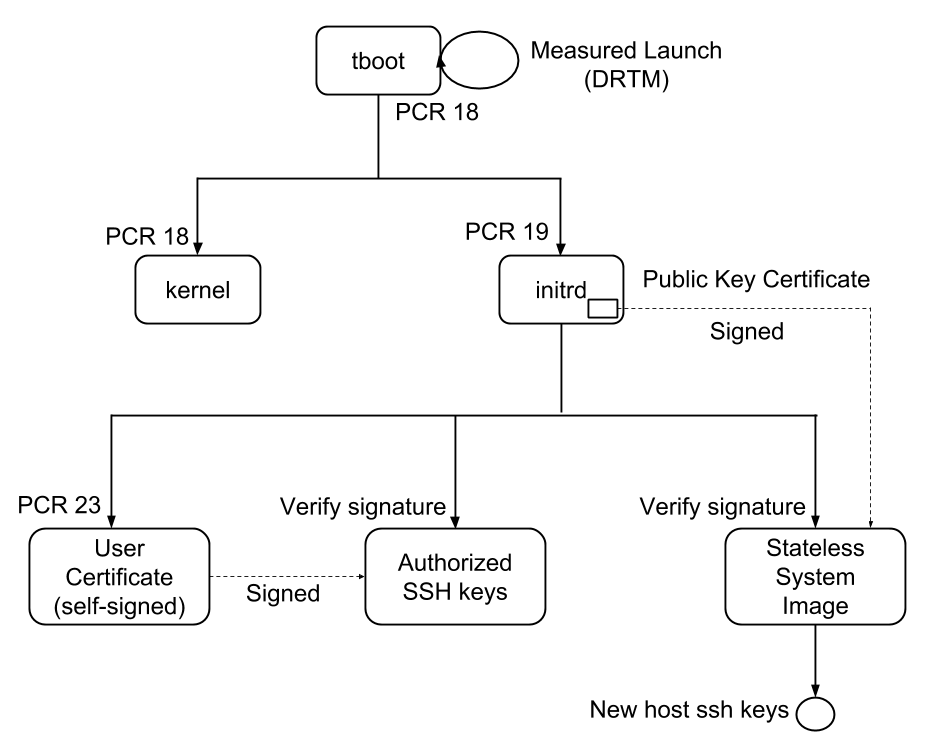
\includegraphics[width=\columnwidth]{drtm}
\centering
\caption{Root of Trust for vCage}
\label{fig-drtm}
\end{figure}

\begin{itemize}
  \item Trusted computing / TPM / TXT
  \item Chain of measurments
    \begin{itemize}
      \item tboot $\to$ kernel $\to$ initrd $\to$ keys
      \item PCR23
    \end{itemize}
  \item Stateless
  \item Keys regenerated on every boot
\end{itemize}

\subsection{System Hardening}
\label{sec:sys-hardening}
Built on a standard Linux kernel, the \vcage\ software cryptoprocessor utilizes various kernel level techniques to increase the security of the system, commonly referred as Linux Kernel Hardening \cite{SANS-hardening:2003}. In this section we describe those techniques in detail, and explain their role in increasing the overall resilience of the system to security threats.

\begin{itemize}
  \item Minimizing the attack surface: \vcage\ uses a minimized Linux kernel, containing a restricted set of system components and drivers. All interfaces to external devices and filesystems are minimal and carefully selected. In order to further close down any endangering communication ports, The only communication protocal that is allowed is SSH.
  \item Enforcing Linux security features: \vcage\ enforces Linux kernel security features including stack canary, Position Independent Executables (PIE), Data Execution Prevention (DEP) and Relocation Read-Only (RELRO) to protect against exploited structures in ELF binaries. Furthermore, it utilizes compilation-time security checks to detect potential string and buffer errors \cite{gcc-fortify}.
  \item Keeping a patched system: Security patches are regularly applied, and custom patches are created when a new vulnerability is disclosed.
  \item Grsecurity ready: Grsecurity is an extensive security enhancenment package to the Linux kernel \cite{Grsec}, incorporating numerous changes and touching nearly 2000 files. Some of its features include mitigation of common memory corruption exploits, Mandatory Access Control system and memory protections for userspace applications.
\end{itemize}

\section{Evaluation}
\label{sec:evaluation}

\begin{itemize}
  \item Real-world use cases
    \begin{itemize}
      \item commercial product
      \item whole-VM protection
      \item availability of compatible systems on cloud providers
    \end{itemize}
  \item More implementation details
  \item Quantitative experiments
\end{itemize}

\subsection{Confidentiality}

\begin{itemize}
  \item Discussion of correctness
  \item Eviction counts for various benchmarks
\end{itemize}

\subsection{Performance}

\begin{itemize}
  \item Discuss modifications to Linux kernel / running VMs on KVM
    \begin{itemize}
      \item Flunky threads
      \item Laptop mode
      \item scan batch sizes
    \end{itemize}

  \item Benchmarks
    \begin{itemize}
      \item Raw memory throughput: 30mb with and w/o privatecore
      \item Crypto benchmark: 30mb with and w/o privatecore
      \item Webserver benchmark: 30mb with and w/o privatecore
      \item Database benchmark: 30mb with and w/o privatecore
    \end{itemize}
\end{itemize}

\section{Related Work}
\label{sec:related}

Related work goes here...

Here are a couple of random cites \cite{Muller:2011wy,Peterson:2010hf} to
test the use of our bibliography file.

\section{Future Work}
\label{sec:future}

\begin{itemize}
  \item Authenticated encryption (Steve)
    \begin{itemize}
      \item GCM performance numbers
      \item Merkle-tree rough design, hit estimate
      \item McGrew dynamic data sets
    \end{itemize}

  \item Future performance optimizations?
  \item Unevictable secrets using address/set mapping?
  \item Anything else?
\end{itemize}

\section{Conclusions}
\label{sec:conclusions}

Conclusions go here...


% Bibliography.
\bibliographystyle{abbrv}
\bibliography{privatecore}

\end{document}
